While the algorithms described in Section~\ref{sec:algorithmDefn} are
ultimately intended for use in a digital fractor, in order to
characterize their frequency response we have simulated them in C++ on a
personal computer. The relative phase as a function of frequency is based upon the
fractional derivative or integral of sinusoidal inputs, sweeping from
low frequency to high frequency in logarithmic steps. Relative phase
is reconstructed using a Numerical Recipes in C algorithm to fit the last
half of the output signal to the sine and cosine components of a
sinusoidal signal with the same frequency as the input signal. From that, phase and amplitude are calculated. 

To verify phase reconstruction, we examine the phase shift of a single
crossing in the time domain for an input frequency of $0.7924$ Hz
(Figures~\ref{fig:timeDomain}). Table~\ref{tab:phaseRecon}
shows a comparison of reconstructed phases using the sinusoidal fit
method and phases obtained from Figure~\ref{fig:timeDomain} by
measuring the phase difference in a single zero-crossing.


\begin{figure}
\begin{center}
\subfigure{
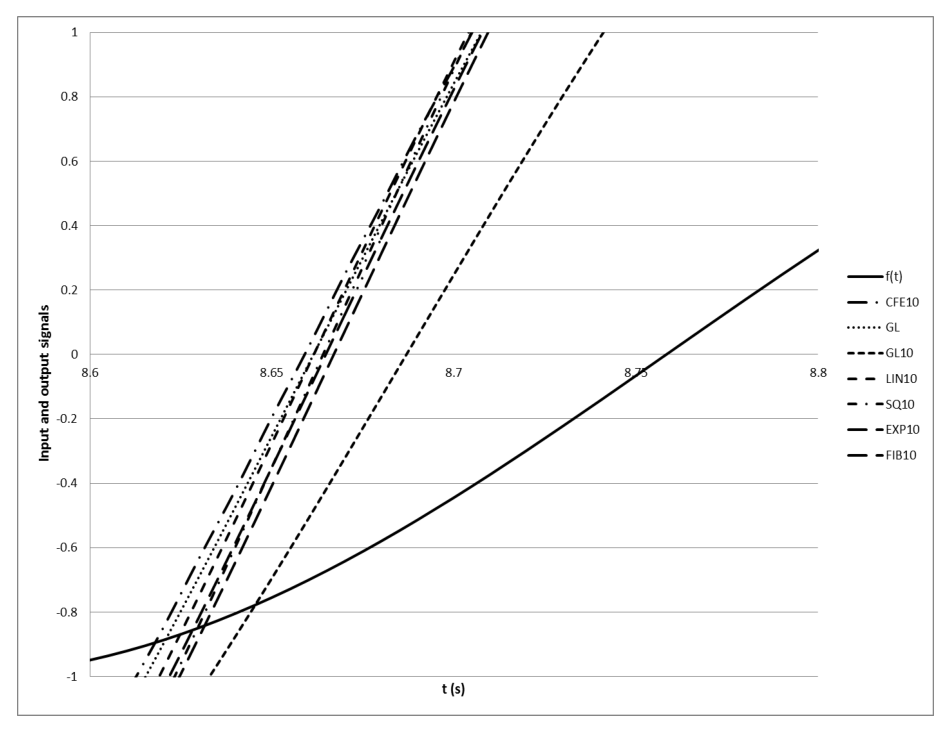
\epsfig{file=timePlotZoom1000_10_10_p05.eps, height=2in,width=2.5in}
}
\subfigure{
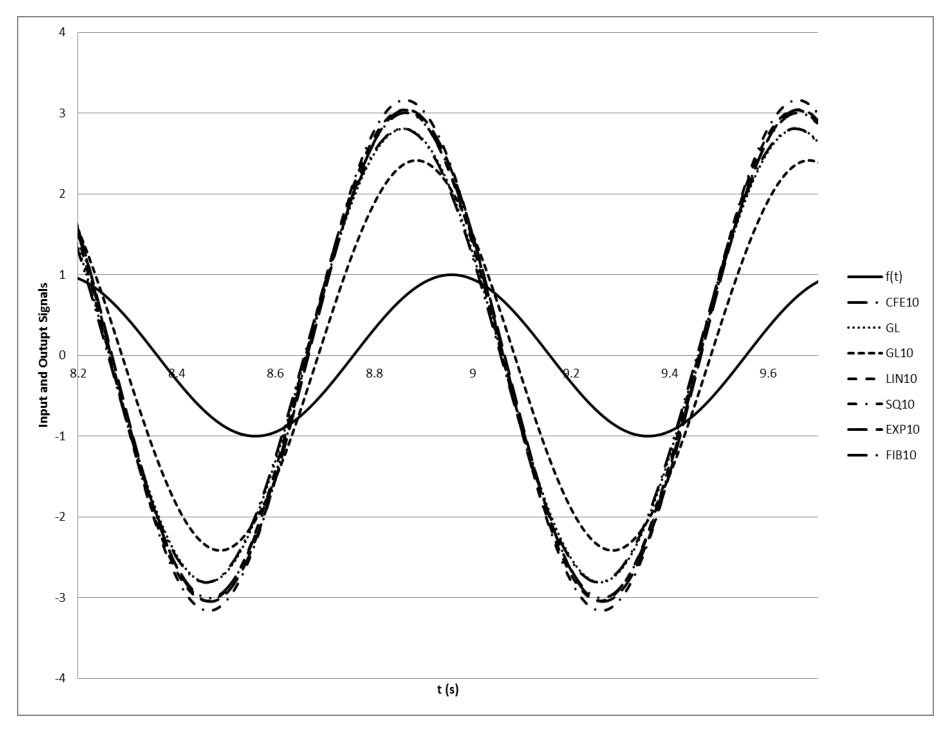
\epsfig{file=timePlot1000_10_10_p05.eps, height=2in,width=2.5in}
}
\end{center}
\caption{Zero crossings of a $0.5$ order derivative of a sine wave input signal
at long times relative to the period. From this the reconstructed
  phase can be verified using the knowledge that the frequency of this
  sine wave was $0.7924$ Hz. Reconstructed and zero-crossing phases
  are shown in Table~\ref{tab:phaseRecon}. In this plot, the duration
  was $10.0$ s and there were $1000$ time steps. There were 10 terms
  in the CFE and 10 bins in all binned Grunwald approximations. A
  variety of binning methods were used: truncated simple Grunwald
  (GL), linearly increasing bin sizes (LIN), bin sizes increasing as a
  square (SQ), exponentially increasing bin sizes (EXP), and bin sizes
  following a Fibonacci rule (FIB).}
\label{fig:timeDomain}
\end{figure}

\begin{table}
\begin{tabular}{llllllll}
\hline
Name &Reconstructed (degrees) &Zero-crossing (degrees)\\ CFE40 &$45.0$
&$45\pm 2$\\ GL &$44.2$ &$41\pm 2$\\ GL26 &$23.0$ &$32\pm 2$\\ LIN26
&$46.1$ &$41\pm 2$\\ SQ26 &$44.4$ &$41\pm 2$\\ EXP26 &$42.1$ &$41\pm
2$\\ FIB26 &$43.0$ &$41\pm 2$\\
\hline
\end{tabular}
\label{tab:phaseRecon}
\caption{Phases reconstructed through sinusoidal fits and phases approximated through single zero-crossings of a single frequency ($0.7924$ Hz) based upon Figure~\ref{fig:zoomTimeDomain}.}
\end{table}

{\bf do we need to say something about amplitude reconstruction?}

The simulation has successfully been run for up to $1,000,000$ time
steps, limited primarily by memory considerations due to the storage
necessary for phase and amplitude reconstruction. At this long
simulation duration, amplitudes and phases over six decades in
frequency are obtained.
